\ifx\allfiles\undefined
\documentclass{article}
\usepackage{amsmath}%换行
\usepackage{ctex}
\usepackage{tikz}
\usepackage{subfigure}
\usepackage{graphicx}
\usepackage{caption}
\usepackage{amsfonts, amssymb}%数学字体

\usepackage{indentfirst} %首行缩进
\makeatletter
\newcommand\figcaption{\def\@captype{figure}\caption} 
\newcommand\tabcaption{\def\@captype{table}\caption}
\renewcommand\figurename{图表} 
\makeatother
\usepackage{float}

\begin{document}

\else

\fi
\chapter{实验研究}
我们对我们的算法进行了广泛的实验研究来评估其有效性,高效性及扩展性。我们在化学分子结构上测试我们的算法。对于化学结构,节点特征包括数值特征和原子布尔特征。数值特征包括元素种类,原子部分电荷,原子电子亲和势,原子自由电子数目和原子价态等等。布尔特征包括原子是否在供体中,是否在末端碳中,是否在环中,是否为负,是否是轴向的等等。在实验中,我们仅用一个原子特征:元素种类。

我们将我们的方法和小波分配核,C-tree,GraphGrep还有gIndex进行比对。我们的算法,WA算法,GraphGrep和gIndex是基于C++实现的,用g++进行编译。C-tree是用Java实现的,用Sun JDK 1.5.0编译。所有的实验都是在Intel Xeon EM64T 3.2GHz,4G内存,Linux系统这一平台上测试的。

WA,G-Hash,C-tree,GraphGrep和gIndex的参数是这样设置的。对于WA和G-hash,h取2,用\emph{haar}小波函数,对于C-tree,用默认值即将最小子节点数m设为20,最大M设为$2m-1$,用NBM方法进行图映射。对于GraphGrep和gIndex,全部采用默认参数。

\section{数据集}
我们选用许多数据集来进行试验。前五个数据集是从从Jorisson/Gilson数据集获得的已有数据。接下来六个是从BindingDB数据集中抽取的,最后一个是NCI/NIH 艾滋病筛选集里的,表1显示了这些数据集和其基本情况。
\subsection{Jorissen数据集}
Jorissen数据集主要为一些包含活动蛋白质的的化学结构信息。我们以药物对特定蛋白质的吸引力作为的目标值。我们选取了5个包含100个分子结构的蛋白质作为测试目标,其中50个化学结构连接着蛋白质,另外50个没连接到蛋白质上。参考文献14来查看详细信息。

\subsection{NCI/NIH AIDS抗体数据库}
NCI/NIH艾滋病抗体数据库包含42390个化学结构,总共有63种分子,最常见的是,C,O,N,S。数据集包括三种边,单边,双边,芬香边。我们选取了所有结构作为数据库,并随机选取1000个化学结构作为查询集合。
\section{利用分类做节点相似性度量}
我们用不同的相似性度量方法比较\emph{k}-NN分类器在Jorissen数据集和BindingDB数据集上的分类精确度。对于WA算法,我们采用小波匹配核函数来获得核矩阵,然后计算距离矩阵来获得最近的k个最相似的图。对于G-Hash,我们根据之前描述的算法计算核函数,然后找出最相似的k个图。对于C-tree,我们直接找回最相似的子图。我们用标准的5-fold交叉验证来获得分类准确度,$(TP+TN)/S$,其中$TP$表示真正结果的数目,$TN$表示真负的数目,$S$是全部的数据图数目。在本实验中,我们取$k=5$。

精确性对比,实验结果如图\ref{fg:ac}所示。可以看出,G-Hash在所有数据集中都比C-tree表现优秀,至少有8\%的提高。G-Hash和C-tree的平均差异大概在13\%。而WA算法较G-Hash表现更为优异,大概有2\%的提升。主要原因是我们简化了距离度量公式。从实验来看,可以明显看出基于核函数的相似性度量方法比基于编辑距离的相似性方法更有优势。因为$k$-NN分类器的精确度和$k$有关,所以我们也研究了不同$k$下算法表现。实验表明精确度对比实验结果不受参数$k$影响。
\begin{figure}[htb]
    \centering
    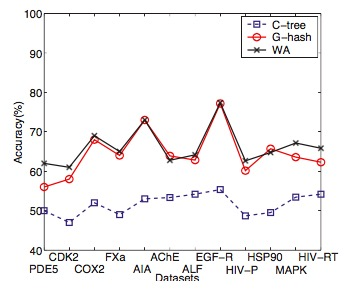
\includegraphics[width=0.5\textwidth]{ac}
    \caption{精确性对比图}
    \label{fg:ac}
\end{figure}
\section{伸缩性}
\subsection{索引构建时间}
我们探究了G-Hash,WA和C-tree,GraphGrep还有gIndex在NCI/NIH艾滋病抗体数据库上的表现。我们比较了不同算法下索引构建时间和索引大小。实验结果如图\ref{fg:bb},\ref{fg:bi}所示。
\begin{figure}[htb]
    \centering
    \begin{minipage}[t]{0.5\textwidth}
        \centering
        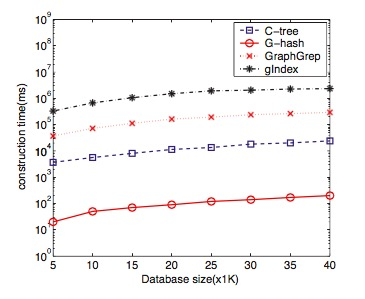
\includegraphics[width=\textwidth]{it}
        \caption{索引构造时间对比图}
        \label{fg:bb}
    \end{minipage}%
    \begin{minipage}[t]{0.5\textwidth}
        \centering
        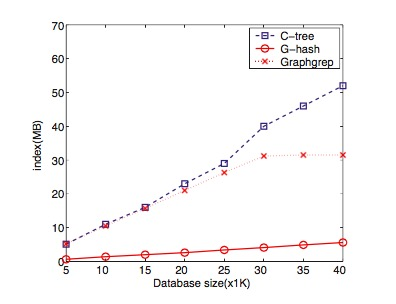
\includegraphics[width=\textwidth]{is}
        \caption{索引大小对比图}
        \label{fg:bi}
    \end{minipage}

\end{figure}

可以看出,无论构建时间,还是索引大小,G-Hash算法均优于其他算法。
\section{查询时间}
我们探究了不同数据库大小对查询时间的影响,实验结果如图\ref{fg:ee}所示。
\begin{figure}[htb]
    \centering
    \begin{minipage}[t]{0.5\textwidth}
        \centering
        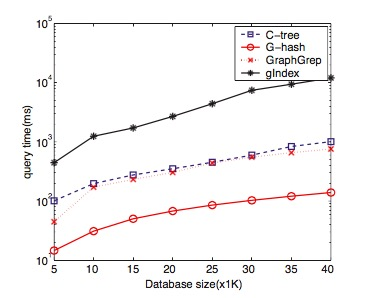
\includegraphics[width=\textwidth]{qt}
        \caption{查询时间和数据库大小关系对比图}
        \label{fg:ee}
    \end{minipage}%
    \begin{minipage}[t]{0.5\textwidth}
        \centering
         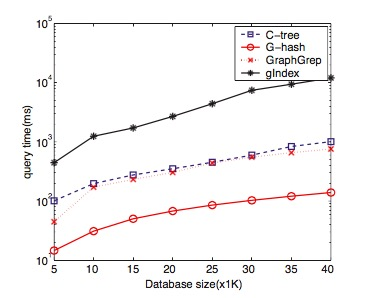
\includegraphics[width=\textwidth]{qt}
        \caption{查询时间和k值关系对比图}
        \label{fg:ek}
    \end{minipage}

\end{figure}

显然,G-Hash比其他算法表现均好,当数据库达到4000时,C-tree,GraphGrep和gIndex的查询时间是G-Hash的8倍,10倍和100倍。

最后我们比较了不同k值下查询时间,如图\ref{fg:ek}所示。


实验表明G-Hash的查询时间与k值的大小没有影响。

\ifx\allfiles\undefined
%\renewcommand\refname{参考文献}
%\bibliographystyle{unsrt}
%\bibliography{G-Hash翻译}
\end{document}
\fi